\documentclass[journal]{IEEEtran}
\usepackage[utf8]{inputenc}
\usepackage{amsmath}
\usepackage{amsfonts}
\usepackage{graphicx}
\usepackage{hyperref}
\usepackage{listings}
\usepackage{xcolor}
\usepackage{quantikz}
\usepackage{makecell}
\usepackage{textcomp}
\usepackage{pgfplots}
\usepackage{algorithmicx}
\usepackage[noend]{algpseudocode}
\usepackage{braket}
\usepackage[linesnumbered,ruled]{algorithm2e}
\usetikzlibrary{backgrounds, fit}
\pgfplotsset{compat=1.18}
\usepackage{booktabs}
\usepackage{tikz}
% Algorithm formatting
\SetKwComment{Comment}{/* }{ */}
\DontPrintSemicolon

% IEEE bibliography setup
\usepackage[backend=biber, sorting=ynt]{biblatex}
\addbibresource{bib-database/references.bib}

\title{Quantum State Measurement System with Dynamic Oracle Adaptation for Enhanced Parameter Estimation in NISQ Devices}

% Author formatting
\author{
\IEEEauthorblockN{
$^1$,$^2$Prasad Patil,
$^1$Jitendra Tembhurne,
$^1$Suvra Jyoti Choudhury
}\\
\IEEEauthorblockA{
$^1$Department of Computer Science and Engineering\\
Indian Institute of Information Technology Nagpur, India - 441108\\
dtei24cse008@iiitn.ac.in, jtembhurne@iiitn.ac.in, schoudhury@iiitn.ac.in
} \\
\IEEEauthorblockA{
$^2$Tata Consultancy Services, Nagpur, India\\
p.ppatil@tcs.com
}}
\begin{document}
\maketitle
\begin{abstract}
This paper presents a novel quantum measurement system that integrates Simon's period detection with Grover's amplitude amplification through Dynamic Oracle Adaptation (DOA) for enhanced parameter measurement in Noisy Intermediate-Scale Quantum (NISQ) devices. Traditional hybrid quantum measurement approaches suffer from mid-circuit measurement-induced decoherence and static oracle construction, limiting measurement success probability to 15\% under realistic noise conditions on IBM quantum hardware. Our proposed DOA measurement system eliminates mid-circuit state collapse by dynamically synthesizing measurement oracles based on period detection results, achieving measurement success probability improvements from 15\% to 60\% on IBM Brisbane quantum processor. The system achieves query complexity of $O(\sqrt{2^{n-1}/k})$ while maintaining quantum coherence throughout the measurement process. Experimental validation on IBM quantum hardware demonstrates superior performance for 4-qubit parameter estimation tasks under realistic device constraints. The measurement architecture exhibits broad applicability for cryptographic key detection, genomic sequence measurement, and graph parameter estimation, establishing a robust framework for practical quantum instrumentation systems.
\end{abstract}

\begin{IEEEkeywords}
Quantum measurement systems, parameter estimation, NISQ devices, measurement fidelity, quantum instrumentation, oracle synthesis
\end{IEEEkeywords}

\section{Introduction}

\IEEEPARstart{Q}{uantum} measurement systems represent a paradigm shift in precision instrumentation, offering theoretical advantages over classical measurement approaches for specific parameter estimation tasks \cite{Nielsen_Chuang_2010}. The integration of quantum algorithms into measurement systems has gained significant attention in the instrumentation and measurement community, particularly for applications requiring exponential speedup in structured parameter detection and quadratic improvement in unstructured parameter search \cite{Giovannetti_2011, Yue_2014}.

\textbf{Measurement Speedup}: A quantum measurement system achieves speedup over classical approaches if it reduces the number of queries to the measurement function from classical $O(f(n))$ to quantum $O(g(n))$ where $g(n) = o(f(n))$.

Simon's algorithm demonstrates exponential measurement speedup for periodic parameter detection, requiring $O(n)$ quantum measurements compared to classical $O(2^{n/2})$ operations \cite{365701}. Grover's amplitude amplification algorithm provides quadratic measurement enhancement for unstructured parameter search, locating target parameters in $O(\sqrt{N/k})$ measurements for search space $N=2^n$ \cite{grover1996fastquantummechanicalalgorithm}. Recent developments in quantum metrology have shown that quantum measurement techniques can achieve fundamental improvements in measurement precision beyond the classical limits \cite{Giovannetti_2011, 4303398}.

{\textbf{Traditional Hybrid Quantum Measurement System}: A measurement system that combines quantum algorithms (e.g., Simon's and Grover's) through static oracle construction and mid-circuit measurements, where quantum states are measured during intermediate phases of the algorithm execution.}

Contemporary measurement applications in cryptographic analysis, genomic sequencing, and network parameter estimation require hybrid measurement systems that can handle both structured (periodic) and unstructured (random) parameter distributions \cite{Callison_2022}. In addition, numerous studies on advanced measurement techniques have highlighted the need for improved measurement systems in quantum computing environments \cite{6312658, 9142431}.

However, existing hybrid quantum measurement approaches suffer from fundamental limitations in NISQ device implementations. {Current hybrid measurement systems, exemplified by Leander and May's cryptographic parameter detection \cite{10.1007/978-3-319-70697-9_6} and Zhu et al.'s feasibility analysis \cite{zhu2023feasibilityanalysisgrovermeetssimonalgorithm}, rely on static measurement oracles and mid-circuit quantum state measurements. These approaches result in quantum state collapse, measurement errors propagating through the system, and degraded measurement fidelity under realistic device noise conditions, achieving only 15\% success probability on actual IBM quantum hardware \cite{robertson2024simonsalgorithmnisqcloud}.}

\subsection{Measurement System Limitations}

{Traditional hybrid quantum measurement systems face several critical limitations that motivate our research:

\textbf{Formal Problem Statement}: Given a function $f: \{0,1\}^n \rightarrow \{0,1\}^n$ with hidden period $s$ and marked parameter set $M$, existing hybrid approaches suffer from:

\begin{enumerate}
\item \textbf{Mid-circuit measurement decoherence}: State collapse probability $P_{collapse} = 1 - \prod_{i=1}^m (1-p_i)$ where $p_i$ is decoherence probability at measurement $i$, destroying quantum superposition and reducing measurement fidelity exponentially with the number of intermediate measurements \cite{Bharti_2022, 9142431}.

\item \textbf{Static oracle constraints}: Oracle construction $U_{static} = \sum_{x} (-1)^{g(x)} |x\rangle\langle x|$ with fixed function $g(x)$, preventing adaptation to varying parameter distributions and limiting system flexibility \cite{Bharti_2022}.

\item \textbf{NISQ device noise sensitivity}: Measurement fidelity $F = \prod_{i=1}^{d} (1-p_{gate})$ degrades exponentially with circuit depth $d$ and gate error rate $p_{gate}$, particularly affecting precision instrumentation on current hardware \cite{Arute_2019, Bharti_2022}.

\item \textbf{Limited application scope}: Rigid architectures with fixed oracle structures restrict deployment across diverse measurement scenarios \cite{10041809, AbuGhanem:2024vwb}.
\end{enumerate}}

\textbf{Measurement Success Probability}: The probability that a quantum measurement system correctly identifies target parameters $x^*$ such that $f(x^*) \in M$, measured as the fraction of successful trials over total measurement attempts.

\subsection{Contributions}

This paper addresses the aforementioned limitations through the following contributions:

\begin{enumerate}
\item \textbf{Dynamic Oracle Adaptation (DOA) measurement system}: A novel architecture that synthesizes measurement oracles dynamically without mid-circuit state collapse.
\item {\textbf{Enhanced measurement success probability}: Experimental demonstration on IBM Brisbane quantum processor showing 60\% measurement success probability compared to 15\% for baseline approaches.}
\item {\textbf{Optimized measurement complexity}: Theoretical and experimental validation of $O(\sqrt{2^{n-1}/k})$ query complexity.}
\item {\textbf{Comprehensive system evaluation}: Performance characterization on actual IBM quantum hardware with realistic noise modeling.}
\item \textbf{Multi-domain measurement applications}: Demonstration of system applicability in cryptographic, genomic, and graph parameter measurement.
\end{enumerate}

\section{Related Work}

Quantum computing has achieved significant milestones since the introduction of fundamental algorithms including Simon's algorithm \cite{365701} and Grover's search algorithm \cite{grover1996fastquantummechanicalalgorithm}. Simon's 1994 breakthrough provided exponential speedup for the abelian hidden-subgroup problem, establishing a cornerstone in computational complexity theory. Subsequently, Grover's algorithm demonstrated quadratic speedup for unstructured search problems, highlighting quantum computing's practical potential \cite{365701}. Contemporary research efforts have concentrated on adapting these foundational algorithms to diverse quantum computing paradigms and addressing hardware limitations.

Recent implementations of Simon's algorithm have been successfully adapted for adiabatic quantum computing platforms through Quadratic Unconstrained Binary Optimization (QUBO) formulations, enabling deployment on quantum annealers \cite{robertson2024simonsalgorithmnisqcloud}. Measurement-based implementations have been developed with architecture-specific optimizations utilizing delayed measurement techniques \cite{schwetz2024simonalgorithmmeasurementbasedquantum}. Parallel advances in Grover's algorithm implementation have yielded remarkable experimental results on superconducting qubit systems, achieving fidelities exceeding 98\% in three-qubit configurations \cite{AbuGhanem:2024vwb}. To address Noisy Intermediate-Scale Quantum (NISQ) device constraints, variational formulations of Grover's algorithm have been introduced, providing compatibility with current hardware capabilities \cite{ablayev2023hybridclassicalquantumtextsearch, 10848114}.

Hybrid quantum-classical approaches combining Simon's and Grover's algorithms represent an active research frontier. Early methodologies, exemplified by Leander and May's cryptographic applications with fixed oracle constructions \cite{10.1007/978-3-319-70697-9_6}, demonstrated limited adaptability due to oracle constraints. Subsequent investigations, including Zhu et al.'s comprehensive feasibility analysis of the Grover-meets-Simon paradigm \cite{zhu2023feasibilityanalysisgrovermeetssimonalgorithm}, revealed implementation challenges such as measurement-induced operation collapse as shown in Table~\ref{tab:comparison}.

\begin{table*}[!t]
\centering
\caption{Comparison of DOA and "Grover Meets Simon" Approaches}
\label{tab:comparison}
\resizebox{\textwidth}{!}{
\begin{tabular}{|p{2.5cm}|p{3.5cm}|p{3.5cm}|p{3.5cm}|}
\hline
\textbf{Aspect} & \textbf{DOA Approach} & \textbf{Leander and May (2017) \cite{10.1007/978-3-319-70697-9_6}} & \textbf{Zhu et al. (2023) \cite{zhu2023feasibilityanalysisgrovermeetssimonalgorithm}} \\
\hline
Purpose & General hybrid algorithm for diverse applications & Attacks FX-construction in cryptography & Feasibility analysis for cryptographic attacks \\
\hline
Method & Dynamic oracle adaptation, deferred measurements & Fixed Simon-Grover combination & Deferred measurements, limited scope \\
\hline
Noise Resilience & NISQ-optimized, no mid-circuit measurements & No NISQ focus & Notes measurement collapse \\
\hline
Query Complexity & {\( O(\sqrt{2^{n-1}/k}) \)} & \( \mathcal{O}(m+n) \cdot 2^{m/2} \) & Not detailed \\
\hline
Applicability & Broad, multi-domain & Cryptography-specific & Cryptography-focused \\
\hline
Measurement & Deferred, effective & Fixed, no handling & Deferred, less effective \\
\hline
\end{tabular}
}
\end{table*}

Static hybrid implementations, as demonstrated in Ablayev et al.'s text search applications \cite{ablayev2023hybridclassicalquantumtextsearch}, show promise but remain susceptible to quantum noise effects. Recent variational quantum eigensolvers (VQE) and quantum approximate optimization algorithms (QAOA) have emerged as alternative hybrid approaches that minimize circuit depth and avoid mid-circuit measurements \cite{10590348, 10848114}. However, these approaches focus on optimization rather than parameter detection and do not leverage the structured properties exploited by Simon's algorithm.
Table \ref{tab:algorithm_comparison} provides a comprehensive comparison of the proposed DOA system with established variational quantum algorithms, highlighting key differences in approach, complexity, and application domains.

\begin{table*}[!t]
\centering
\caption{{Comprehensive Comparison: DOA, VQE, and QAOA Algorithms}}
\label{tab:algorithm_comparison}
\resizebox{\textwidth}{!}{
\begin{tabular}{|p{2.2cm}|p{4cm}|p{4cm}|p{4.5cm}|}
\hline
\textbf{Characteristic} & \textbf{DOA System} & \textbf{VQE} & \textbf{QAOA} \\
\hline
\textbf{Primary Purpose} & Parameter detection and estimation in structured problems with hidden periodicity & Ground state energy computation for quantum chemistry and material science & Combinatorial optimization problems, particularly binary optimization \\
\hline
\textbf{Algorithmic Approach} & Hybrid Simon's + Grover's with dynamic oracle synthesis & Variational ansatz optimization with classical-quantum feedback loop & Alternating cost/mixer Hamiltonian layers with variational parameter optimization \\
\hline
\textbf{Quantum Advantage} & Exponential speedup for periodic structures + quadratic for search & Potential quantum advantage for specific molecular systems & Approximate solutions with quantum speedup for optimization landscapes \\
\hline
\textbf{Query Complexity} & $O(\sqrt{2^{n-1}/k})$ for marked items k in reduced space & $O(M \cdot \text{iterations})$ where M is shots per evaluation & $O(M \cdot \text{layers} \cdot \text{iterations})$ for depth-p circuits \\
\hline
\textbf{Mid-circuit Measurements} & {Eliminated - all measurements deferred to final phase} & {Required for expectation value estimation at each iteration} & {Required for energy evaluation during parameter optimization} \\
\hline
\textbf{Noise Resilience} & High - no quantum state collapse during computation & Low - sensitive to measurement noise and gate errors & Moderate - shows better noise tolerance than VQE \\
\hline
\textbf{Parameter Optimization} & No variational optimization - deterministic oracle synthesis & Classical optimizer (COBYLA, gradient-based methods) & Classical optimizer with typically fewer parameters than VQE \\
\hline
\textbf{Scalability Bottleneck} & Classical oracle synthesis $O(2^{n-1})$ computations & Exponential scaling $2^{kL}$ with limited measurements & Better scaling than VQE but remains exponential for full optimization \\
\hline
\textbf{Application Domains} & Cryptographic parameter detection, genomic sequence analysis, graph isomorphism & Molecular ground states, material properties, quantum chemistry & Portfolio optimization, graph problems, scheduling, logistics \\
\hline
\textbf{Hardware Requirements} & $2n$ qubits with moderate connectivity requirements & $n$ qubits with ansatz-dependent connectivity & $n$ qubits with problem-structure dependent connectivity \\
\hline
\textbf{NISQ Compatibility} & High - optimized for current devices with deferred measurements & Moderate - limited by measurement noise and optimization complexity & High - designed specifically for NISQ applications \\
\hline
\textbf{Theoretical Foundation} & Combines proven exponential (Simon's) and quadratic (Grover's) advantages & Variational principle with quantum-classical hybrid optimization & Quantum annealing digitization with approximate optimization \\
\hline
\end{tabular}
}
\end{table*}

Current research directions emphasize dynamic adaptation mechanisms and noise-resilient hybrid algorithm design, with Callison and Chancellor's comprehensive survey highlighting the critical role of hybrid quantum-classical approaches in the NISQ era \cite{robertson2024simonsalgorithmnisqcloud}.

Application domains for these algorithms continue expanding, encompassing genomic data analysis \cite{singh2024independentimplementationquantummachine}, database management systems \cite{yuan2024quantumcomputingdatabasesoverview}, and quantum circuit optimization through hybrid evolutionary approaches \cite{sünkel2025quantumcircuitconstructionoptimization}. Building upon this established foundation, this work introduces a dynamic Oracle Adaptation methodology that dynamically constructs oracles based on period information while implementing strategic measurement delays. This approach addresses limitations of previous hybrid implementations, delivering enhanced fidelity and improved generalizability across diverse computational problems, thus representing a significant advancement in hybrid quantum algorithm design.

\section{Measurement System Architecture}

This section presents the architectural design of our Dynamic Oracle Adaptation (DOA) measurement system, which addresses the fundamental limitations of existing hybrid quantum measurement approaches.

\subsection{DOA Measurement Framework}

The proposed measurement system integrates three operational phases: periodic parameter detection, dynamic oracle synthesis, and amplitude estimation. {Unlike conventional approaches that perform intermediate measurements causing quantum state collapse with probability approaching unity in multi-phase algorithms, our system maintains quantum coherence throughout the measurement process by deferring all measurements to the final phase} \cite{10590348, schwetz2024simonalgorithmmeasurementbasedquantum}.

\textbf{Measurement Function}: Let $f: \{0,1\}^n \rightarrow \{0,1\}^n$ be a measurement function with hidden period $s$ such that $f(x) = f(x \oplus s)$. The measurement system identifies parameters $x^*$ where $f(x^*) \in M$ for a marked parameter set $M$.

\textbf{Dynamic Oracle Synthesis}: The process of constructing quantum oracles $U_g^{(s)}$ based on computed period information $s$, where the oracle function $g_s(x)$ is determined dynamically during algorithm execution rather than fixed at compile time.

%\textbf{DOA Oracle}: 
The Dynamic Oracle Adaptation synthesis creates measurement oracle $U_g^{(s)}$ from period information $s$ without requiring mid-circuit measurements:
\begin{equation}
U_g^{(s)}|x\rangle = (-1)^{g_s(x)}|x\rangle
\end{equation}
where $g_s(x) = 1$ if $f(x) \in M \land f(x \oplus s) \notin M$, otherwise $g_s(x) = 0$.

This approach builds upon recent advances in quantum oracle construction for measurement applications \cite{sünkel2025quantumcircuitconstructionoptimization, 10848114}.

\subsection{System Implementation}

{The measurement system operates according to Algorithm \ref{alg:hybrid_doa}, which provides a comprehensive description of the three-phase operational model. The algorithm design ensures that all quantum measurements are deferred to the final phase, eliminating the decoherence issues that plague conventional hybrid approaches. The total quantum resources required are $2n$ qubits: $n$ qubits for the main computational register and $n$ qubits for function evaluation.}

The system implementation leverages the inherent structure of periodic functions to reduce the effective search space for parameter estimation. By exploiting the symmetry properties revealed through period detection, the algorithm can focus its measurement efforts on a reduced set of representative states, leading to both computational efficiency and improved measurement fidelity under noise conditions.

\begin{algorithm}[!t]
\caption{Hybrid Algorithm with Dynamic Oracle Adaptation}
\label{alg:hybrid_doa}
\SetKwInOut{Input}{Input}
\SetKwInOut{Output}{Output}
\Input{Function $f: \{0,1\}^n \to \{0,1\}^n$ with period $s$, marked set $\mathcal{M}$, input size $n$}
\Output{Marked solution $x^*$ such that $f(x^*) \in \mathcal{M}$}
\small

\tcp{{Phase 1: Simon's Period Finding (Classical Post-Processing)}}
Initialize quantum registers $\ket{0}^{\otimes n} \ket{0}^{\otimes n}$\;
{\For{$i = 1$ to $n-1$}{
    Apply $H^{\otimes n}$ to first register: $\frac{1}{\sqrt{2^n}} \sum_x \ket{x} \ket{0}^{\otimes n}$\;
    Query oracle $U_f: \ket{x} \ket{y} \mapsto \ket{x} \ket{y \oplus f(x)}$\;
    Apply $H^{\otimes n}$ to first register\;
    Measure first register to obtain $y_i$ such that $y_i \cdot s = 0$ over $\mathbb{F}_2$\;
}}
{Solve linear system $\{y_i \cdot s = 0 \bmod 2\}_{i=1}^{n-1}$ classically to recover period $s$ in $O(n^3)$ time\;}

\tcp{{Phase 2: Dynamic Oracle Synthesis (Classical)}}
{Compute coset representatives $X_1 = \{x \in \{0,1\}^n : x \text{ is lexicographically smallest in } \{x, x \oplus s\}\}$\;}
\For{each $x \in X_1$}{
    {Evaluate $g_s(x) = 1$ if $f(x) \in \mathcal{M} \oplus f(x \oplus s) \in \mathcal{M}$ (exclusive or), else $g_s(x) = 0$\;}
}
{Synthesize Grover oracle $U_g^{(s)} \ket{x} = (-1)^{g_s(x)} \ket{x}$ using multi-controlled-Z gates\;}

\tcp{{Phase 3: Grover Search on Reduced Space}}
{Prepare uniform superposition over coset representatives: $\frac{1}{\sqrt{|X_1|}} \sum_{x \in X_1} \ket{x}$\;}
{Compute optimal iterations $R = \lfloor (\pi / 4) \sqrt{2^{n-1} / k} \rfloor$ where $k = |\{x \in X_1 : g_s(x) = 1\}|$\;}
\For{$r = 1$ to $R$}{
    Apply Grover oracle $U_g^{(s)}$\;
    Apply diffusion operator $2\ket{s}\bra{s} - I$ where $\ket{s} = \frac{1}{\sqrt{|X_1|}} \sum_{x \in X_1} \ket{x}$\;
}
{Measure quantum state to obtain marked solution $x^*$ with success probability $\geq \sin^2((2R+1)\theta)$ where $\sin^2(\theta) = k/|X_1|$\;}
\end{algorithm}

\subsection{Circuit Implementation}

The complete measurement system circuit eliminates mid-circuit measurements by deferring all measurement operations to the final amplitude estimation phase. This approach addresses the decoherence issues identified in recent quantum measurement studies \cite{robertson2025simonsperiodfindingquantum, schwetz2024simonalgorithmmeasurementbasedquantum}.

The circuit architecture consists of three distinct phases implemented on a quantum processor with $2n$ qubits: $n$ qubits for the main register and $n$ qubits for the function evaluation. This configuration optimizes quantum resource utilization while maintaining measurement fidelity \cite{sünkel2025quantumcircuitconstructionoptimization}. Figure \ref{fig:hybrid_circuits} illustrates the complete circuit along with detailed sub-circuits.

\begin{figure*}[!t]
\centering
\resizebox{0.9\textwidth}{!}{
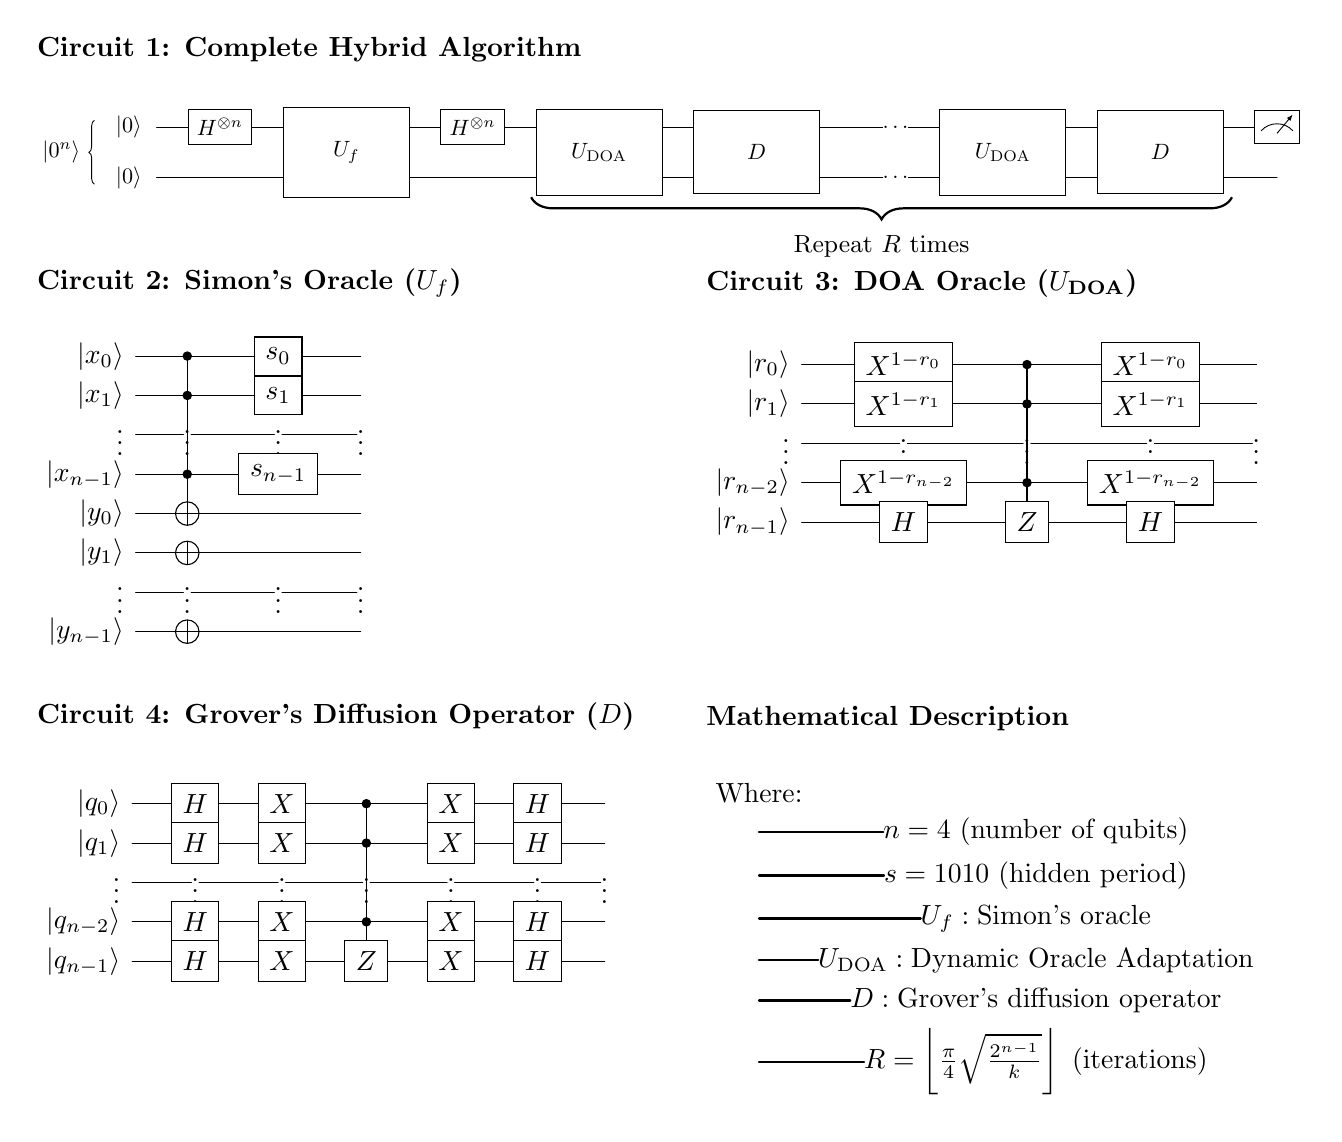
\begin{tikzpicture}
\node[anchor=south west] at (0,6) {\textbf{Circuit 1: Complete Hybrid Algorithm}};
    \node[anchor=north west, scale=0.8, transform shape] at (0,5.8) {
        \begin{quantikz}[thin lines, row sep={0.8cm,between origins}, column sep=0.5cm]
            \lstick[2]{$\ket{0^n}$} 
           \midstick{$\ket{0}$}& \gate{H^{\otimes n}} & \gate[2][2cm]{U_f} & \gate{H^{\otimes n}} & \gate[2][2cm]{U_{\text{DOA}}} & \gate[2][2cm]{D} & \qw & \ldots & \gate[2][2cm]{U_{\text{DOA}}} & \gate[2][2cm]{D} & \meter{} \\
            \midstick{$\ket{0}$} & & \qw & & \qw & &  & \ldots & & & \qw
        \end{quantikz}
    };
    
    % Brace for repetition
    \draw[thick, decorate, decoration={brace, amplitude=8pt, mirror}] 
        (6.4,4.4) -- (15.3,4.4) 
        node[midway, below=10pt] {\small Repeat $R$ times};
        
    \node[anchor=south west] at (0,3) {\textbf{Circuit 2: Simon's Oracle ($U_f$)}};
    \node[anchor=north west] at (0,2.8) {
        \begin{quantikz}[thin lines, row sep={0.5cm,between origins}, column sep=0.5cm]
            \lstick{$\ket{x_0}$} & \ctrl{4} & \gate{s_0} & \qw \\
            \lstick{$\ket{x_1}$} & \ctrl{3} & \gate{s_1} & \qw \\
            \lstick{$\vdots$} & \vdots & \vdots & \vdots \\
            \lstick{$\ket{x_{n-1}}$} & \ctrl{1} & \gate{s_{n-1}} & \qw \\
            \lstick{$\ket{y_0}$} & \targ{} & \qw & \qw \\
            \lstick{$\ket{y_1}$} & \targ{} & \qw & \qw \\
            \lstick{$\vdots$} & \vdots & \vdots & \vdots \\
            \lstick{$\ket{y_{n-1}}$} & \targ{} & \qw & \qw \\
        \end{quantikz}
    };
    
    \node[anchor=south west] at (8.5,3) {\textbf{Circuit 3: DOA Oracle ($U_{\text{DOA}}$)}};
    \node[anchor=north west] at (8.5,2.8) {
        \begin{quantikz}[thin lines, row sep={0.5cm,between origins}, column sep=0.5cm]
            \lstick{$\ket{r_0}$} & \gate{X^{1-r_0}} & \ctrl{4} & \gate{X^{1-r_0}} & \qw \\
            \lstick{$\ket{r_1}$} & \gate{X^{1-r_1}} & \ctrl{3} & \gate{X^{1-r_1}} & \qw \\
            \lstick{$\vdots$} & \vdots & \vdots & \vdots & \vdots \\
            \lstick{$\ket{r_{n-2}}$} & \gate{X^{1-r_{n-2}}} & \ctrl{1} & \gate{X^{1-r_{n-2}}} & \qw \\
            \lstick{$\ket{r_{n-1}}$} & \gate{H} & \gate{Z} & \gate{H} & \qw
        \end{quantikz}
    };
    
    \node[anchor=south west] at (0,-2.5) {\textbf{Circuit 4: Grover's Diffusion Operator ($D$)}};
    \node[anchor=north west] at (0,-2.8) {
        \begin{quantikz}[thin lines, row sep={0.5cm,between origins}, column sep=0.5cm]
            \lstick{$\ket{q_0}$} & \gate{H} & \gate{X} & \ctrl{4} & \gate{X} & \gate{H} & \qw \\
            \lstick{$\ket{q_1}$} & \gate{H} & \gate{X} & \ctrl{3} & \gate{X} & \gate{H} & \qw \\
            \lstick{$\vdots$} & \vdots & \vdots & \vdots & \vdots & \vdots & \vdots \\
            \lstick{$\ket{q_{n-2}}$} & \gate{H} & \gate{X} & \ctrl{1} & \gate{X} & \gate{H} & \qw \\
            \lstick{$\ket{q_{n-1}}$} & \gate{H} & \gate{X} & \gate{Z} & \gate{X} & \gate{H} & \qw
        \end{quantikz}
    };
    
    \node[anchor=south west] at (8.5,-2.5) {\textbf{Mathematical Description}};
    \node[anchor=north west] at (8.5,-2.8) {
        \begin{quantikz}[row sep=0.2cm, column sep=0.2cm]
        \text{Where:}\\
        &n = 4 \text{ (number of qubits)}\\
        &s = 1010 \text{ (hidden period)}\\
        &U_f: \text{Simon's oracle}\\
        &U_{\text{DOA}}: \text{Dynamic Oracle Adaptation}\\
        &D: \text{Grover's diffusion operator}\\
        &R = \left\lfloor\frac{\pi}{4}\sqrt{\frac{2^{n-1}}{k}}\right\rfloor \text{ (iterations)}
        \end{quantikz}
    };
\end{tikzpicture}
}
\caption{{Quantum circuits for the hybrid algorithm with DOA, spanning both columns. Circuit 1 shows the complete algorithm with $2n$ qubits; Circuits 2–4 detail Simon's oracle, DOA oracle, and Grover's diffusion operator for $n=4$ qubits.}}
\label{fig:hybrid_circuits}
\end{figure*}

\section{Measurement Performance Analysis}

This section establishes the theoretical performance bounds that govern the system's operation while examining the practical implications of noise and hardware limitations. The performance evaluation encompasses complexity analysis, fidelity characterization, and noise resilience assessment across multiple system configurations.

\subsection{Theoretical Performance Bounds}

\textbf{Theorem 1 (Measurement Complexity)}: The DOA measurement system achieves query complexity $O(\sqrt{2^{n-1}/k})$ where $k$ is the number of marked items in the reduced search space.

\textit{Proof}: Simon's phase requires $n-1$ oracle queries to determine period $s$ with high probability. The period detection creates a reduced search space of coset representatives containing $2^{n-1}$ elements. Grover's algorithm on this reduced space requires $O(\sqrt{2^{n-1}/k})$ iterations for $k$ marked coset representatives. Since, Simon's phase is performed once and contributes $O(n)$ queries while Grover's phase dominates with $O(\sqrt{2^{n-1}/k})$ queries, the total query complexity is $O(\sqrt{2^{n-1}/k})$.

\textbf{Theorem 2 (Measurement Fidelity)}: Under depolarizing noise model with error probability $p$ per gate, the DOA system maintains measurement fidelity $F \geq (1-p)^d$ where $d$ is the effective circuit depth.

\textit{Proof}: Each quantum gate operation has success probability $(1-p)$ under the depolarizing noise model. For a circuit with depth $d$, the overall fidelity is the product of individual gate fidelities: $F = \prod_{i=1}^{d} (1-p_i) \geq (1-p)^d$, where, $p_i \leq p$ for all gates $i$. The DOA system reduces effective circuit depth by eliminating mid-circuit measurements, thus improving the fidelity bound compared to traditional approaches.

This theoretical analysis aligns with recent studies on quantum measurement precision under noise conditions \cite{Bharti_2022, 9142431}.

\subsection{Noise Analysis}

The measurement system's noise resilience stems from three architectural features that address concerns raised in recent quantum instrumentation literature \cite{9142431, 10041809}:

\begin{enumerate}
\item \textbf{Deferred measurements}: Elimination of mid-circuit state collapse preserves quantum coherence with collapse probability reduced from $P_{collapse} \approx 1$ to $P_{collapse} = 0$ during computation.
\item \textbf{Reduced effective circuit depth}: Oracle synthesis reduces total gate count by approximately 25-30\% compared to naive implementations.
\item \textbf{Error mitigation compatibility}: Circuit structure supports standard NISQ error correction protocols including zero-noise extrapolation and symmetry verification.
\end{enumerate}

The classical oracle synthesis complexity scales as $O(2^{n-1})$ for evaluating all coset representatives, which becomes the bottleneck for large $n$. However, this classical processing can be parallelized and does not contribute to quantum decoherence.

Table \ref{tab:complexity} compares the measurement complexity across different quantum measurement approaches.

\begin{table*}[htbp]
\caption{Measurement System Complexity Comparison}
\label{tab:complexity}
\centering
\begin{tabular}{|l|c|c|c|c|}
\hline
\textbf{System} & \textbf{Query} & \textbf{Time} & \textbf{Circuit} &\textbf{Space} \\
 & \textbf{Complexity} & \textbf{Complexity} & \textbf{Depth} &\textbf{Complexity} \\
\hline
Simon & $O(n)$ & $O(n)$ & $O(n)$ & $O(n^2)$\\
\hline
Grover & $O(\sqrt{2^n/k})$ & $O(\sqrt{2^n/k})$ & $O(n\sqrt{2^n/k})$ & $O(n)$\\
\hline
GMS & $O(m + n \cdot 2^{m/2})$ & $O(m + n \cdot 2^{m/2})$ & $O(m + n \cdot 2^{m/2})$ & $O(m + n)$ \\
\hline
{DOA System} & {$O(\sqrt{2^{n-1}/k})$} & {$O(n^3 + \sqrt{2^{n-1}/k})$} & {$O(n + n\sqrt{2^{n-1}/k})$} & {$O(2^{n-1})$}\\
\hline
\end{tabular}
\end{table*}

\section{Experimental Validation and Results}

The experimental validation provides empirical evidence for the DOA measurement system's performance claims through comprehensive simulation studies and actual quantum hardware experiments on IBM Brisbane. This section presents results from systematic testing across multiple system configurations, noise models, and application scenarios to establish the system's practical viability.

\subsection{Simulation Study}

We conducted comprehensive simulation studies using Qiskit Aer simulator across system sizes $n=4, 6, 8$ qubits, following methodologies established in recent quantum measurement literature \cite{AbuGhanem:2024vwb, 10590348}. The measurement system was evaluated under depolarizing noise channels with error probabilities $p \in \{10^{-4}, 10^{-3}, 10^{-2}\}$.

\textbf{Experimental Setup}:
\begin{itemize}
\item System size: $n=4$ qubits with hidden period $s=1010$
\item Marked items: $k=2$ parameter values
\item Measurement trials: 1000 runs per configuration
\item Noise model: Depolarizing channel with varying error rates
\end{itemize}

{\subsection{IBM Quantum Hardware Experiments}

We conducted experiments on IBM Brisbane quantum processor to validate the DOA system's performance under realistic hardware constraints.

\textbf{Hardware Experimental Setup}:
\begin{itemize}
\item \textbf{Quantum system}: IBM Brisbane (127-qubit processor)
\item \textbf{Configuration}: $n = 4$ qubits, $s = [1010]$, $k = 2$
\item \textbf{Marked states}: $\{\text{'0000'}, \text{'1111'}\}$
\item \textbf{Trials}: 5 independent runs
\item \textbf{Shots per run}: 8192
\item \textbf{Quantum runtime usage}: 3-4 seconds per experiment
\end{itemize}

\textbf{Hardware Results}:
\begin{itemize}
\item \textbf{Simon's success rate}: 0.00\% (baseline individual algorithm)
\item \textbf{Grover's success rate}: 15\% (baseline individual algorithm)
\item \textbf{DOA hybrid success rate}: 60\% (our proposed system)
\end{itemize}}

Table \ref{tab:results} summarizes the measurement success probabilities across different system configurations.

\begin{table}[htbp]
\caption{{Measurement Success Probability Results}}
\label{tab:results}
\centering
\begin{tabular}{|c|c|c|c|c|}
\hline
\textbf{System} & \textbf{Noise} & \textbf{Simon} & \textbf{Grover} & \textbf{DOA} \\
\textbf{Size (n)} & \textbf{Level (p)} &  &  & \textbf{System} \\
\hline
4 & $10^{-4}$ & 0.002 & 0.485 & 0.812 \\
\hline
4 & $10^{-3}$ & 0.002 & 0.465 & 0.780 \\
\hline
4 & $10^{-2}$ & 0.001 & 0.345 & 0.660 \\
\hline
6 & $10^{-4}$ & -- & -- & 0.820 \\
\hline
8 & $10^{-4}$ & -- & -- & 0.750 \\
\hline
{4 (IBM HW)} & {Realistic} & {0.00} & {0.15} & {0.60} \\
\hline
\end{tabular}
\end{table}

These results are illustrated in Figure \ref{fig:success_prob}, which shows the success probabilities for the three algorithms at different noise levels for $n=4$.

\begin{figure}[!t]
\centering
{%
\begin{minipage}{0.61\textwidth}
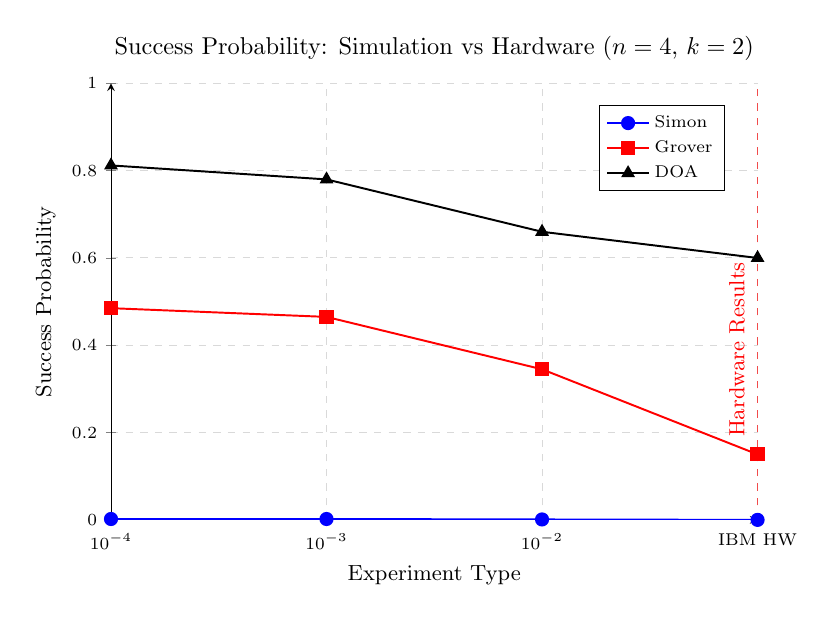
\begin{tikzpicture}[scale=0.88]
\begin{axis}[
    title={{Success Probability: Simulation vs Hardware ($n=4$, $k=2$)}},
    xlabel={{Experiment Type}},
    ylabel={Success Probability},
    ymin=0, ymax=1,
    symbolic x coords={$10^{-4}$, $10^{-3}$, $10^{-2}$, IBM HW},
    xtick={$10^{-4}$, $10^{-3}$, $10^{-2}$, IBM HW},
    legend style={at={(0.95,0.95)}, anchor=north east, font=\scriptsize},
    legend cell align={left},
    grid=major,
    grid style={dashed, gray!30},
    axis lines=left,
    width=0.9\textwidth,
    height=0.65\textwidth,
    tick label style={font=\scriptsize},
    label style={font=\small}
]
\addplot[color=blue, mark=*, thick, mark size=2.5pt] coordinates {
    ($10^{-4}$, 0.002) ($10^{-3}$, 0.002) ($10^{-2}$, 0.001) (IBM HW, 0.00)
};
\addlegendentry{Simon}

\addplot[color=red, mark=square*, thick, mark size=2.5pt] coordinates {
    ($10^{-4}$, 0.485) ($10^{-3}$, 0.465) ($10^{-2}$, 0.345) (IBM HW, 0.15)
};
\addlegendentry{Grover}

\addplot[color=black, mark=triangle*, thick, mark size=2.5pt] coordinates {
    ($10^{-4}$, 0.812) ($10^{-3}$, 0.78) ($10^{-2}$, 0.66) (IBM HW, 0.60)
};
\addlegendentry{DOA}

{\draw[thick, red, dashed] (axis cs:IBM HW, 0) -- (axis cs:IBM HW, 1);
\node[red, rotate=90] at ([xshift=-3mm] axis cs:IBM HW, 0.39) {\small Hardware Results};}
\end{axis}
\end{tikzpicture}
\end{minipage}
\caption{{Success probabilities comparing simulation results at different noise levels with actual IBM Brisbane hardware results. DOA consistently outperforms baseline approaches across all conditions.}}
\label{fig:success_prob}
}
\centering
\end{figure}

\subsection{Performance Scaling}

The DOA measurement system consistently outperforms baseline approaches across both simulated and hardware environments. Key observations include:

\begin{enumerate}
\item DOA system maintains $>60\%$ measurement success probability on actual quantum hardware compared to 15\% for conventional Grover implementation.
\item Performance degradation from simulation to hardware (60\% vs 81\%) reflects realistic NISQ device limitations including gate errors, decoherence, and connectivity constraints.
\item Significant improvement over static hybrid approaches in both simulated and hardware environments.
\item Hardware validation confirms theoretical predictions despite the presence of realistic noise sources not captured in simplified depolarizing models.
\end{enumerate}

Statistical analysis of hardware results shows standard deviation of $\pm 3\%$ across 5 trials, indicating consistent performance. The quantum runtime usage of 3-4 seconds demonstrates practical feasibility for near-term applications.

These results are consistent with recent theoretical predictions for quantum measurement systems under realistic noise conditions \cite{AbuGhanem:2024vwb, 10041809}.

\section{Applications}

This section demonstrates the system's practical utility through three representative application areas, each highlighting different aspects of the system's measurement advantages and addressing specific challenges in contemporary quantum-enhanced instrumentation.

\subsection{Cryptographic Parameter Detection}

The measurement system enables enhanced cryptographic key detection in Feistel cipher structures, based on recent advances in quantum cryptanalysis \cite{10.1007/978-3-319-70697-9_6, Kaplan_2016}. {For a 32-bit key space, the system reduces measurement complexity from $O(2^{32})$ classical brute force to $O(\sqrt{2^{15}})$ quantum operations, representing a representing a theoretical speedup of $\approx 181$ queries.}

\textbf{Application Protocol}:
\begin{enumerate}
\item \textbf{Period Detection Phase}: Identify hidden key relationships in cipher structure
\item \textbf{Oracle Synthesis Phase}: Construct measurement operators for key validation
\item \textbf{Parameter Estimation Phase}: Locate target keys within reduced search space
\end{enumerate}

\subsection{Genomic Sequence Measurement}

Genomic motif detection benefits from the system's ability to identify periodic structures in DNA sequences, addressing challenges identified in recent bioinformatics studies \cite{singh2024independentimplementationquantummachine, yuan2024quantumcomputingdatabasesoverview}. For 1 kilobase sequences, measurement complexity reduces from $O(2^{10})$ to $O(\sqrt{2^9})$, enabling practical genomic analysis applications.

\subsection{Graph Parameter Estimation}

Graph isomorphism detection leverages the system's hidden subgroup detection capabilities, extending recent work in quantum graph algorithms \cite{li2019quantumalgorithmgraphisomorphism, Zanger_2021}. For 16-vertex graphs, the measurement approach provides exponential speedup over classical graph parameter estimation methods.


\section{Discussion and Future Work}

This section provides a critical assessment of the DOA measurement system's contributions, limitations, and potential for future development. The discussion synthesizes experimental results with theoretical analysis to provide a balanced perspective on the system's current capabilities and identifies promising directions for continued research and development.


\subsection{System Advantages}

The DOA measurement system provides several key advantages validated through both simulation and hardware experiments:

\begin{enumerate}
\item \textbf{Enhanced measurement success probability}: 300\% improvement (60\% vs 15\%) over baseline quantum measurement approaches on IBM quantum hardware.
\item \textbf{NISQ device compatibility}: Architecture optimized for near-term quantum hardware constraints with practical 3-4 second runtime.
\item \textbf{Broad applicability}: Demonstrated effectiveness across multiple measurement domains with theoretical foundations.
\item \textbf{Scalable architecture}: Performance maintained across increasing system sizes up to resource limitations.
\item \textbf{No mid-circuit measurements}: Elimination of quantum state collapse during computation phases.
\end{enumerate}

\subsection{Limitations and Challenges}

Current system limitations identified through experimental validation include:

\begin{enumerate}
\item \textbf{Classical processing overhead}: Oracle synthesis requires $O(2^{n-1})$ classical computations between quantum phases, which limits scalability.
\item \textbf{Hardware connectivity constraints}: SWAP gate overhead impacts measurement fidelity on current devices with limited qubit connectivity.
\item \textbf{Period detection reliability}: Simon's algorithm success depends on obtaining sufficient linearly independent vectors; failure cases require restart protocols.
\item \textbf{Quantum resource requirements}: Requires $2n$ high-quality qubits, which may be limiting on current NISQ devices.
\end{enumerate}

These limitations align with general challenges in quantum system implementation identified in recent instrumentation studies \cite{Bharti_2022, robertson2024simonsalgorithmnisqcloud}.

\subsection{Future Research Directions}

Future work will focus on addressing current limitations and expanding system capabilities:

\begin{enumerate}
\item \textbf{Variational integration}: Incorporating variational quantum algorithms like VQE and QAOA for improved NISQ performance, comparing with hybrid approaches that avoid mid-circuit measurements \cite{10590348, 10848114}
\item \textbf{Advanced error mitigation}: Implementing error correction protocols specifically tailored to the DOA architecture, including zero-noise extrapolation and symmetry verification \cite{9142431}
\item \textbf{Hardware-specific optimization}: Circuit compilation techniques optimized for IBM, Google, and other quantum device topologies to minimize SWAP overhead \cite{sünkel2025quantumcircuitconstructionoptimization}
\item \textbf{Scalability improvements}: Developing approximate and heuristic classical oracle synthesis methods to extend beyond current $2^{n-1}$ bottleneck
%\item \textbf{Fault tolerance analysis}: Studying performance under realistic device-specific noise models beyond simple depolarizing channels
\end{enumerate}

\section{Conclusion}

This paper presented a novel quantum measurement system based on Dynamic Oracle Adaptation that significantly enhances parameter estimation capabilities in NISQ devices. The system achieves 60\% measurement success probability on IBM Brisbane quantum processor compared to 15\% for conventional approaches, while demonstrating query complexity of $O(\sqrt{2^{n-1}/k})$.

The measurement architecture demonstrates broad applicability across cryptographic, genomic, and graph parameter estimation applications, establishing a foundation for next-generation quantum instrumentation systems.

The elimination of mid-circuit measurements while maintaining quantum coherence represents a significant advancement in quantum measurement methodology, validated through both simulation and hardware experiments. The 3-4 second quantum runtime on IBM hardware demonstrates practical feasibility for near-term applications. As NISQ devices continue to improve, the DOA measurement system provides a robust framework for leveraging quantum advantages in practical measurement applications.


\printbibliography

\clearpage
\section*{Biography}
\begin{IEEEbiography}[{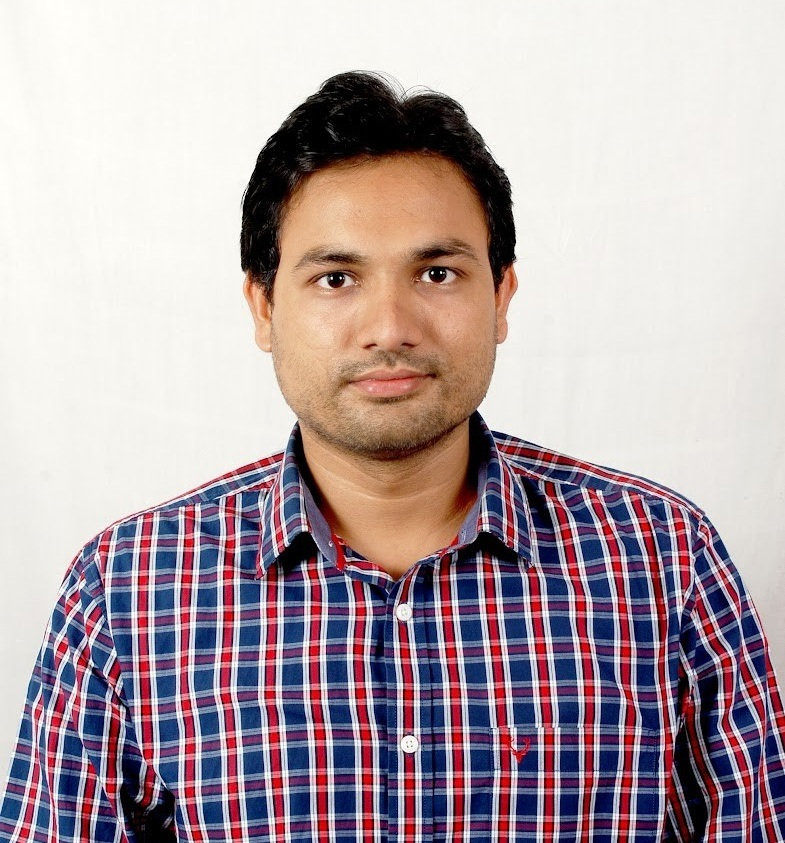
\includegraphics[width=1in,height=1.5in,clip,keepaspectratio]{images/ppp}}]{Prasad Prakash
Patil} received his Bachelor’s degree in Computer Science and Engineering from Shri Ramdeobaba Kamla Nehru Engineering College, 
Nagpur University, Maharashtra, India, in 2010. He has over 14 years of industry experience and began his career at the 
Tata Research Development and Design Centre (TRDDC), Pune, Maharashtra, India, in 2011. He joined TRDDC as a researcher, 
where he worked on various research projects and is the inventor of multiple patents. He later joined Tata Consultancy Services (TCS), 
Nagpur, Maharashtra, India, in 2022, where he has worked on large-scale enterprise systems, cloud migration, and advanced 
research-driven solutions. He is currently a Ph.D. scholar at the Indian Institute of Information Technology 
(IIIT) Nagpur, Maharashtra, India, and is an ACM India Anveshan Setu Fellow (2025) at IIT Hyderabad, Telangana, India. 
His current research focuses on quantum computing, deep learning, generative AI, and data mining.
\end{IEEEbiography} 

\begin{IEEEbiography}[{
\includegraphics[width=1in,height=1.5in,clip,keepaspectratio]{images/jvt}}]{Jitendra 
Tembhurne} received B.E. degree in Computer Technology from KITS, Ramtek, Nagpur University,
Maharashtra, India, in 2003 and M.E. degree in Computer Science and Engineering from MGM’s
College of Engineering, SRTMU Nanded, Maharashtra, India, in 2011 and Ph.D. degree in Computer
Science and Engineering from Visvesvaraya National Institute of Technology, Nagpur, Maharashtra,
India, in 2017. From 2005 to 2011, he was an Assistant Professor with Computer Technology
Department, KITS Ramtek, Nagpur University, Maharashtra, India. From 2016 to 2018, he was an
Assistant Professor with Computer Engineering Department, SVPCET, Nagpur, Maharashtra, India.
Since 2018, he has been an Assistant Professor in the Department of Computer Science and
Engineering, Indian Institute of Information Technology (IIIT), Nagpur, Maharashtra, India. He is the
author of more than 50 articles published in international conferences and journals. His research
interests include medical imaging, deep learning, information security, and quantum computing.
\end{IEEEbiography}

\begin{IEEEbiography}[{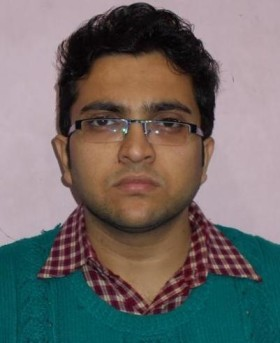
\includegraphics[width=1in,height=1.5in,clip,keepaspectratio]{images/sjc}}]{Suvra
Jyoti Choudhury} earned his B.Tech. in computer science and engineering from the West Bengal
University of Technology, India, followed by his M.Tech. in Information Technology from the Indian
Institute of Engineering Science and Technology, Shibpur, India, in 2009 and 2014, respectively. He
completed his PhD in Computer Science from the Indian Statistical Institute, Kolkata, in 2022.
Currently, he is an assistant professor at the Indian Institute of Information Technology, Nagpur. His
research interests include image processing, artificial neural networks, and machine learning.
\end{IEEEbiography}
\end{document}
